\documentclass{article}

\usepackage{graphicx}
\usepackage{tikz}
\usepackage{tikzsymbols}
\usetikzlibrary{calc,patterns,shapes.geometric}
\pagestyle{empty}
\usepackage[margin=0pt]{geometry}
\geometry{papersize={14in,12in}}

\def\centerarc[#1](#2)(#3:#4:#5){\draw[#1] ($(#2)+({#5*cos(#3)},{#5*sin(#3)})$) arc (#3:#4:#5);}

\begin{document}
	\begin{figure}
		\centering
		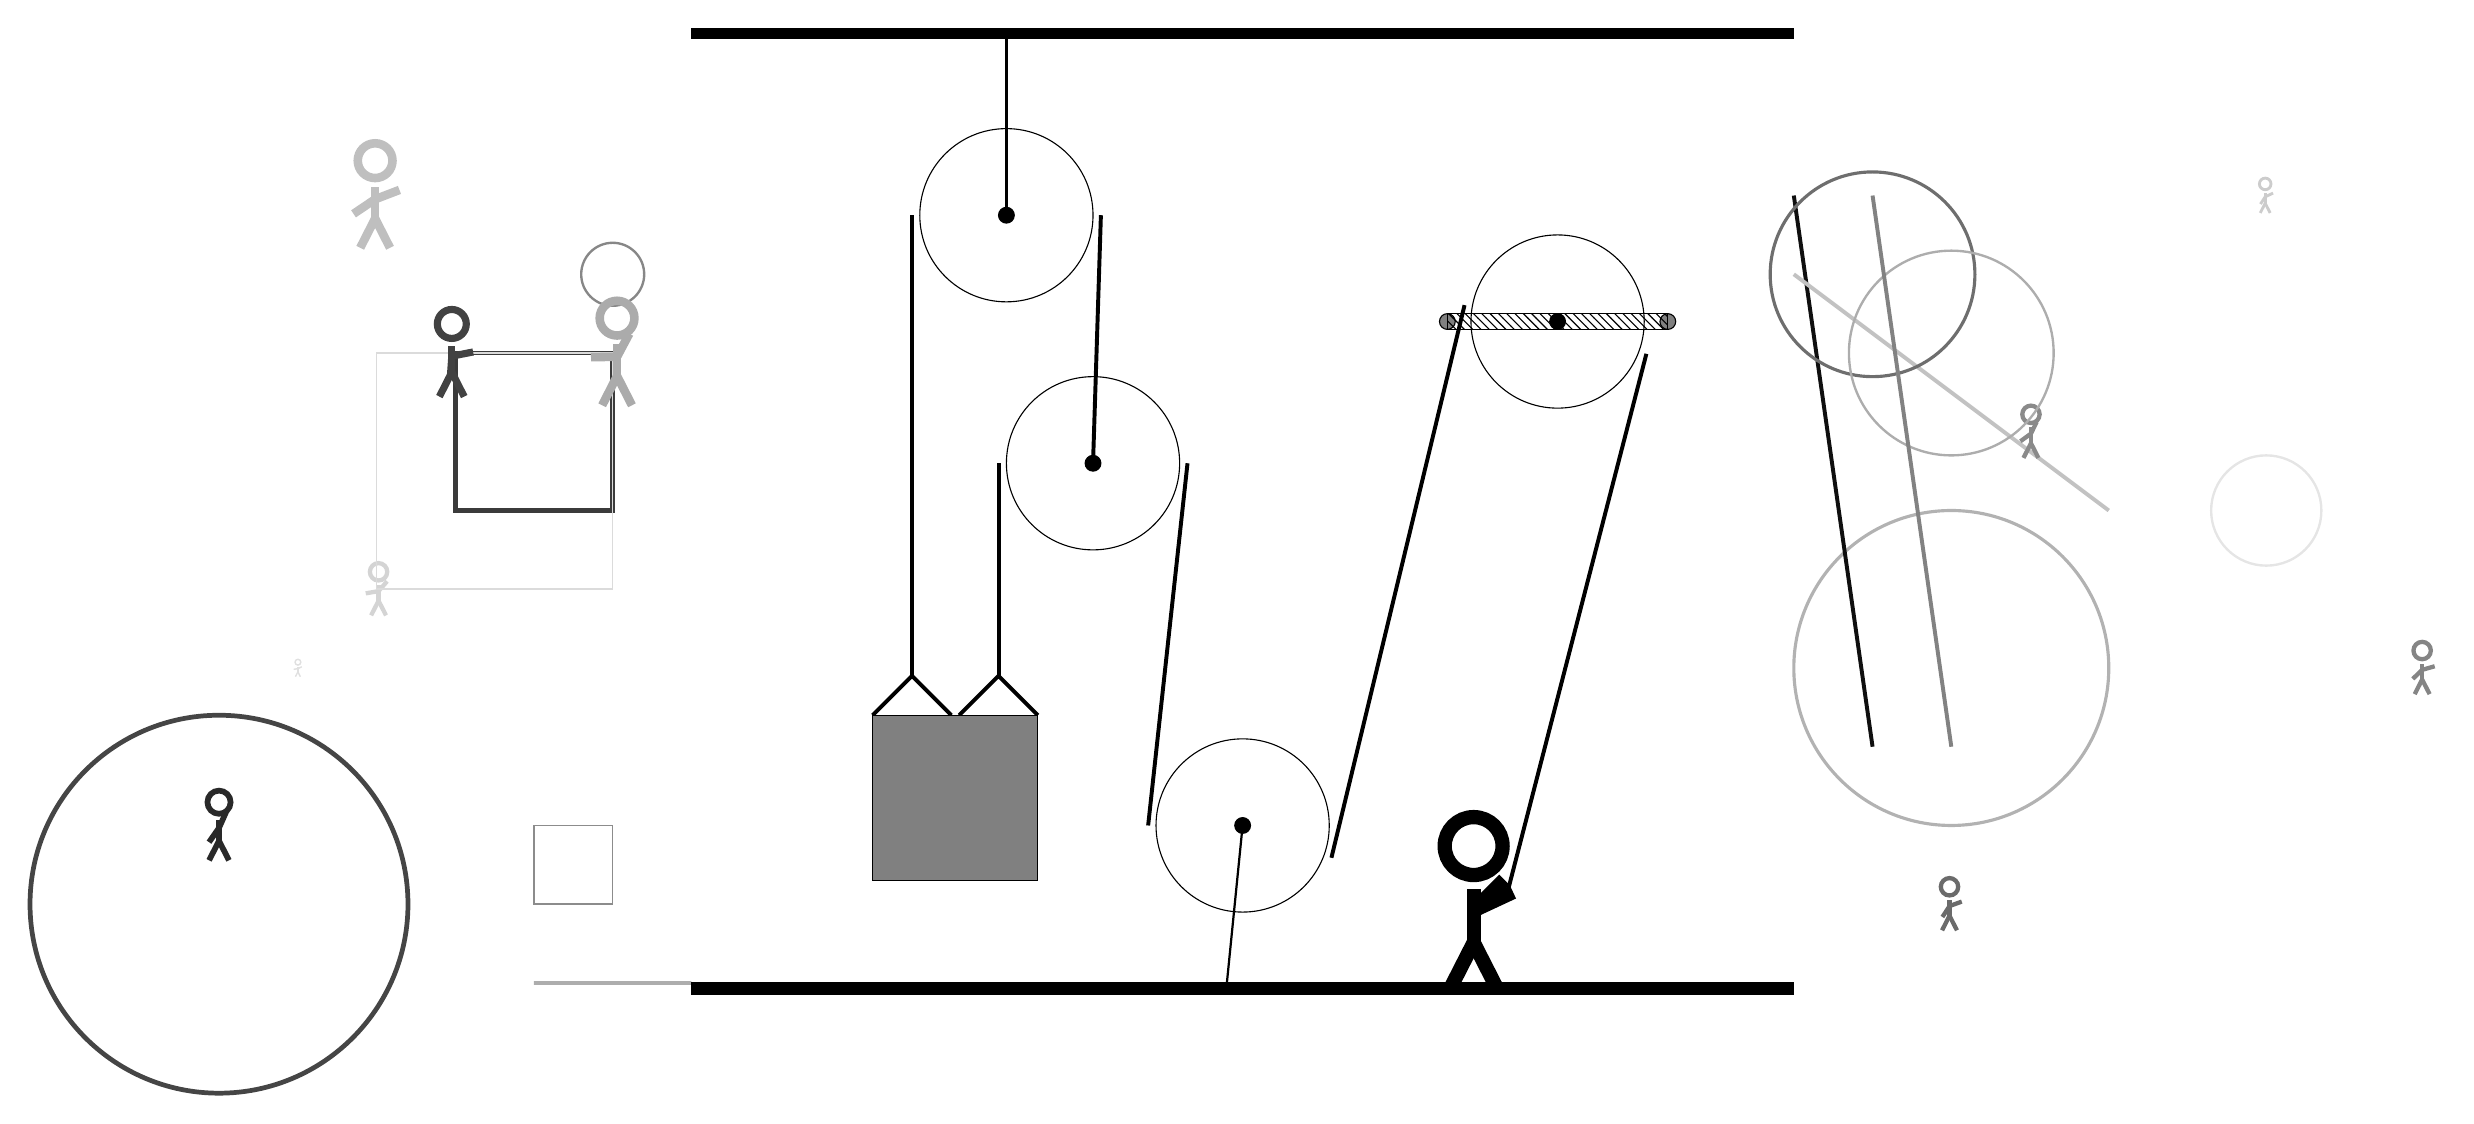
\begin{tikzpicture}
			%%%%% START %%%%%
			
			\draw[fill=black] (-2, 9) rectangle (12, 9.125);
			
			\draw (2, 6.75) circle (1.1);
			\draw[fill=black] (2, 6.75) circle (0.1);
			\draw[thick] (2, 6.75) -- (2, 9);
			
			\draw (3.1, 3.6) circle (1.1);
			\draw[fill=black] (3.1, 3.6) circle (0.1);
			
			\node[line width=0.5mm, color=black!48] at (20, 1) {\Strichmaxerl[3][44][16]};
			
			\draw[line width=0.2mm, color=black!45] (-4, -2) rectangle (-3, -1);
			\draw [line width=0.3mm, color=black!47](-3, 6) circle (0.4);
			\draw[line width=0.6mm, color=black!77] (-3, 3) rectangle (-5, 5);
			\node[line width=0.3mm, color=black!17] at (-6, 2) {\Strichmaxerl[3][10][49]};
			\draw [line width=0.4mm, color=black!30](14, 1) circle (2.0);
			\draw [line width=0.6mm, color=black!73](-8, -2) circle (2.4);
			\draw [line width=0.3mm, color=black!10](18, 3) circle (0.7);
			\draw[line width=0.5mm, color=black!94](12, 7) -- (13, 0);
			\node[line width=0.5mm, color=black!12] at (-7, 1) {\Strichmaxerl[1][10][25]};
			
			\draw[line width=0.2mm, color=black!14] (-3, 5) rectangle (-6, 2);
			\node[line width=0.6mm, color=black!33] at (-3, 5) {\Strichmaxerl[6][1][62]};
			\node[line width=0.3mm, color=black!25] at (-6, 7) {\Strichmaxerl[6][34][21]};
			
			\node[line width=0.4mm, color=black!74] at (-5, 5) {\Strichmaxerl[5][86][11]};
			\node[line width=0.5mm, color=black!84] at (-8, -1) {\Strichmaxerl[4][55][66]};
			\draw[line width=0.5mm, color=black!32] (-4, -3) rectangle (-2, -3);
			
			\draw[line width=0.5mm, color=black!24](12, 6) -- (16, 3);
			\node[line width=0.2mm, color=black!20] at (18, 7) {\Strichmaxerl[2][57][25]};
			\draw [line width=0.4mm, color=black!57](13, 6) circle (1.3);
			\node[line width=0.4mm, color=black!46] at (15, 4) {\Strichmaxerl[3][36][64]};
			\node[line width=0.7mm, color=black!58] at (14, -2) {\Strichmaxerl[3][57][20]};
			\draw [line width=0.3mm, color=black!32](14, 5) circle (1.3);
			\draw[line width=0.5mm, color=black!49](13, 7) -- (14, 0);
			
			\draw (5, -1) circle (1.1);
			\draw[fill=black] (5, -1) circle (0.1);
			\draw[thick] (5, -1) -- (4.8, -3);
			
			\draw (9, 5.4) circle (1.1);
			\draw[fill=black] (9, 5.4) circle (0.1);
			\draw[fill=black!50] (7.6, 5.4) circle (0.1);
			\draw[fill=black!50] (10.4, 5.4) circle (0.1);
			\draw[pattern=north west lines, pattern color=black] (7.6, 5.5) rectangle (10.4, 5.3);
			
			\draw[line width = 0.5mm]  (0.3, 0.4) -- (0.8, 0.9) -- (1.3, 0.4);
			\draw[line width = 0.5mm]  (1.4, 0.4) -- (1.9, 0.9) -- (2.4, 0.4);
			\draw[fill=black!50] (0.3, 0.4) rectangle (2.4, -1.7);
			
			\draw[line width = 0.5mm] (0.8, 6.75) -- (0.8, 0.9);
			\centerarc[line width = 0.5mm](2, 6.75)(0:180:1.2000000000000002);
			\draw[line width = 0.5mm] (3.2, 6.75) -- (3.1, 3.6);
			\draw[line width = 0.5mm] (1.9, 3.6) -- (1.9, 0.9);
			\centerarc[line width = 0.5mm](3.1, 3.6)(0:180:1.2000000000000002);
			\draw[line width = 0.5mm] (4.3, 3.6) -- (3.8, -1);
			\centerarc[line width = 0.5mm](5, -1)(180:340:1.2000000000000002);
			\draw[line width=0.5mm](6.1276, -1.4104) -- (7.8182, 5.6083);
			\centerarc[line width = 0.5mm](9, 5.4)(-20:170:1.2000000000000002);
			\draw[line width=0.5mm](10.1276, 4.9896) --  (8.35, -1.9);
			
			\node at (8, -2) {\Strichmaxerl[10][225][25]};
			
			\draw[fill=black] (-2, -3) rectangle (12, -3.15);
			
			%%%%% END %%%%%
		\end{tikzpicture}
	\end{figure}	
\end{document}